\capitulo{6}{Trabajos relacionados}

El análisis del proceso de diseño en entornos de modelado tridimensional ha despertado un interés creciente durante los últimos años, especialmente en ámbitos como la arquitectura, la ingeniería, la educación y la interacción persona-computador. Este interés se fundamenta en la posibilidad de registrar automáticamente las interacciones del usuario con herramientas digitales, generando conjuntos de datos que permiten estudiar el comportamiento de diseño desde una perspectiva objetiva, empírica y cuantificable~\cite{gao2021,gao2023,jankowski2014}.

Con el objetivo de estructurar de forma sistemática el estado del arte, las investigaciones analizadas se han agrupado en cuatro líneas fundamentales:
\begin{enumerate}
    \item Análisis basado en registros de eventos (\textit{event logs}) y minería de procesos (\textit{process mining}).
    \item Estudios empíricos sobre el comportamiento y la pericia del diseñador.
    \item Adquisición de datos en entornos virtuales e inmersivos.
    \item Aplicaciones pedagógicas y educativas del modelado 3D.
\end{enumerate}

\section{Análisis del proceso de diseño mediante \textit{event logs}}

Una de las líneas de investigación más relevantes se centra en el uso de registros de eventos generados automáticamente por herramientas de modelado 3D~\cite{gao2021,liu2022}. Estos registros permiten capturar de forma automatizada las acciones realizadas por el usuario durante el proceso de diseño.

Gao et al.~\cite{gao2021} proponen una estructura de datos basada en grafos para modelar la relación entre comandos y objetos durante el proceso de modelado. Este enfoque permite analizar secuencias de acciones y comprender la lógica subyacente del proceso de diseño. Posteriormente, Gao et al.~\cite{gao2023} amplían esta línea mediante técnicas de \textit{process mining}, demostrando que es posible identificar patrones de comportamiento y relacionarlos con la creatividad del diseño.

De forma complementaria, Liu et al.~\cite{liu2022} aplican estos principios en contextos educativos, mostrando que los \textit{event logs} permiten reconstruir el proceso de diseño de los estudiantes y analizar su evolución. Asimismo, Xie et al.~\cite{xie2014} utilizan análisis de series temporales sobre datos de diseño asistido por computador para evaluar el comportamiento del diseñador y detectar patrones iterativos durante el proceso de modelado.

\textbf{Limitación:} La mayoría de estos trabajos se centran principalmente en el análisis estadístico diferido (\textit{a posteriori}) de los datos y en entornos específicos y rígidos como BIM o CAD, careciendo de herramientas integradas en entornos de modelado generalistas que permitan la recopilación analítica no intrusiva.

\section{Estudios sobre comportamiento del diseñador}

Otra línea de investigación se orienta a comprender cómo trabajan los diseñadores y cómo varía su comportamiento en función de su experiencia y nivel de pericia~\cite{casakin2023,chen2022,welch}.

Chen et al.~\cite{chen2022} analizan las diferencias entre diseñadores expertos y novatos, identificando variaciones significativas en las estrategias jerárquicas utilizadas durante el proceso de diseño. En la misma línea, Casakin y Levy~\cite{casakin2023} proponen un marco formal para medir el comportamiento del diseñador experto, identificando factores correlacionados con la descomposición del problema y el uso de pensamiento conceptual. Por su parte, Welch y Lim~\cite{welch} demuestran que los diseñadores novatos suelen adoptar procesos más iterativos, erráticos y menos estructurados que los diseñadores con mayor experiencia técnica.

\textbf{Limitación:} Estos trabajos se basan fundamentalmente en análisis experimentales controlados o estudios teóricos con muestras de datos reducidas y técnicas intrusivas de observación directa (como protocolos de pensamiento en voz alta), lo que limita su escalabilidad, automatización y aplicación en entornos reales de producción.

\section{Entornos virtuales e inmersivos}

El avance de las tecnologías inmersivas ha abierto nuevas posibilidades para el análisis del comportamiento del usuario durante tareas de diseño tridimensional~\cite{krassmann2018,wang2024}.

Wang et al.~\cite{wang2024} presentan un análisis a gran escala del comportamiento de diseño en entornos de realidad virtual, utilizando datos de interacción y posicionamiento para modelar automáticamente el proceso de diseño. De forma similar, Krassmann et al.~\cite{krassmann2018} estudian el comportamiento de usuarios en entornos virtuales mediante técnicas de seguimiento óculo-manual y visualización interactiva.

\textbf{Limitación:} Estos enfoques dependen estrictamente de hardware dedicado y plataformas inmersivas de realidad mixta, lo que restringe su aplicabilidad directa en las herramientas de modelado de propósito general y pantallas tradicionales que dominan la industria actual.

\section{Aplicaciones educativas del modelado 3D}

El modelado 3D también constituye un recurso ampliamente extendido en contextos educativos y formativos de disciplinas técnicas y artísticas~\cite{koh2010,sosna2025}.

Sosna et al.~\cite{sosna2025} demuestran que el uso de herramientas de modelado tridimensional favorece el desarrollo de la cognición espacial y la creatividad en estudiantes de diseño. Asimismo, Koh et al.~\cite{koh2010} evidencian que las simulaciones y la manipulación tridimensional mejoran la motivación intrínseca y el rendimiento académico durante los procesos de aprendizaje técnico complejo.

\textbf{Limitación:} Aunque estas investigaciones demuestran los beneficios pedagógicos del modelado 3D, la mayoría de los enfoques abordados no profundizan en la captura estructurada de las mallas ni en el análisis analítico y geométrico detallado de la interacción del usuario.

\section{Comparación y posicionamiento del presente trabajo}

A partir del análisis de la literatura científica, se observa que las soluciones existentes presentan avances significativos en la conceptualización del proceso de diseño, aunque persisten brechas metodológicas importantes en lo que respecta a la captura automatizada en tiempo real y la integración nativa dentro de herramientas de modelado generalistas.

Las principales limitaciones identificadas en el estado del arte se sintetizan en los siguientes puntos:
\begin{itemize}
    \item Dependencia de análisis externos realizados de forma diferida, impidiendo una evaluación contextual inmediata.
    \item Confinamiento a entornos propietarios de tipo CAD/BIM o plataformas inmersivas costosas.
    \item Ausencia de integración con el flujo topológico interno (mallas y mapas UV) en software de propósito general.
    \item Uso de metodologías de monitorización intrusivas que alteran la experiencia de usuario o degradan el rendimiento del sistema operativo.
\end{itemize}

La Tabla~\ref{tab:comparativa_trabajos} resume comparativamente las características funcionales de los trabajos analizados frente a la solución propuesta en este proyecto.

\begin{table}[H]
\centering
\small
\begin{tabular}{lcccc}
\hline
\textbf{Trabajo} & \textbf{Adquisición TR} & \textbf{Generalista} & \textbf{No intrusivo} & \textbf{Análisis geométrico} \\
\hline
Gao et al. (2021)       &   &   & X & X \\
Gao et al. (2023)       &   &   & X & X \\
Liu et al. (2022)       &   &   & X & X \\
Xie et al. (2014)       &   &   & X & X \\
Chen et al. (2022)      & X &   &   & X \\
Casakin et al. (2023)   & X &   &   & X \\
Wang et al. (2024)      &   &   &   & X \\
Krassmann et al. (2018) &   &   &   & X \\
Sosna et al. (2025)     & X & X &   &   \\
Koh et al. (2010)       & X & X &   &   \\
\textbf{Add-on Blender 1.0} & \textbf{X} & \textbf{X} & \textbf{X} & \textbf{X} \\
\hline
\end{tabular}
\caption{Comparativa entre trabajos relacionados y el sistema desarrollado en el presente proyecto.}
\label{tab:comparativa_trabajos}
\end{table}

\textit{Nota aclaratoria sobre la Tabla~\ref{tab:comparativa_trabajos}:} El sistema desarrollado garantiza la adquisición de eventos en tiempo real (TR) mediante \textit{handlers} asíncronos de fondo, mientras que la generación de visualizaciones estadísticas complejas se ejecuta bajo demanda para preservar la tasa de refresco gráfica del entorno.

La Figura~\ref{fig:estado_arte_posicionamiento} representa el espacio tridimensional conceptual en el que se posiciona esta investigación con respecto a las soluciones previas de la literatura.

\begin{figure}[H]
\centering
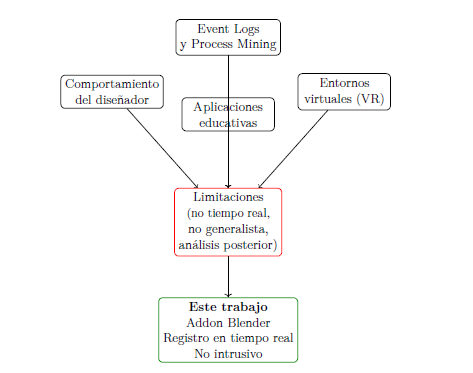
\includegraphics[
    width=\textwidth,
    height=0.65\textheight,
    keepaspectratio
]{diagramas/arte.png}
\caption{Resumen del estado del arte y posicionamiento del trabajo desarrollado.}
\label{fig:estado_arte_posicionamiento}
\end{figure}

La principal aportación del sistema integrado \textit{Add-on Blender 1.0} radica en su capacidad para unificar la adquisición no intrusiva de interacciones y el análisis topológico avanzado directamente dentro de una plataforma de uso extendido en la industria como Blender. Al mitigar las limitaciones de los enfoques tradicionales, este proyecto proporciona un marco funcional que extrae variables de mallas estructurales, calcula índices complejos como la distancia de Hausdorff y proyecta analíticas visuales en el propio espacio tridimensional, constituyendo una herramienta versátil tanto para la auditoría profesional como para la investigación educativa.